\documentclass[10pt,]{article}
\usepackage{lmodern}
\usepackage{amssymb,amsmath}
\usepackage{ifxetex,ifluatex}
\usepackage{fixltx2e} % provides \textsubscript
\ifnum 0\ifxetex 1\fi\ifluatex 1\fi=0 % if pdftex
  \usepackage[T1]{fontenc}
  \usepackage[utf8]{inputenc}
\else % if luatex or xelatex
  \ifxetex
    \usepackage{mathspec}
    \usepackage{xltxtra,xunicode}
  \else
    \usepackage{fontspec}
  \fi
  \defaultfontfeatures{Mapping=tex-text,Scale=MatchLowercase}
  \newcommand{\euro}{€}
\fi
% use upquote if available, for straight quotes in verbatim environments
\IfFileExists{upquote.sty}{\usepackage{upquote}}{}
% use microtype if available
\IfFileExists{microtype.sty}{%
\usepackage{microtype}
\UseMicrotypeSet[protrusion]{basicmath} % disable protrusion for tt fonts
}{}
\usepackage[margin=1in]{geometry}
\ifxetex
  \usepackage[setpagesize=false, % page size defined by xetex
              unicode=false, % unicode breaks when used with xetex
              xetex]{hyperref}
\else
  \usepackage[unicode=true]{hyperref}
\fi
\hypersetup{breaklinks=true,
            bookmarks=true,
            pdfauthor={pm/bm},
            pdftitle={ISOR Coding Procedures},
            colorlinks=true,
            citecolor=blue,
            urlcolor=blue,
            linkcolor=magenta,
            pdfborder={0 0 0}}
\urlstyle{same}  % don't use monospace font for urls
\usepackage{color}
\usepackage{fancyvrb}
\newcommand{\VerbBar}{|}
\newcommand{\VERB}{\Verb[commandchars=\\\{\}]}
\DefineVerbatimEnvironment{Highlighting}{Verbatim}{commandchars=\\\{\}}
% Add ',fontsize=\small' for more characters per line
\usepackage{framed}
\definecolor{shadecolor}{RGB}{248,248,248}
\newenvironment{Shaded}{\begin{snugshade}}{\end{snugshade}}
\newcommand{\KeywordTok}[1]{\textcolor[rgb]{0.13,0.29,0.53}{\textbf{{#1}}}}
\newcommand{\DataTypeTok}[1]{\textcolor[rgb]{0.13,0.29,0.53}{{#1}}}
\newcommand{\DecValTok}[1]{\textcolor[rgb]{0.00,0.00,0.81}{{#1}}}
\newcommand{\BaseNTok}[1]{\textcolor[rgb]{0.00,0.00,0.81}{{#1}}}
\newcommand{\FloatTok}[1]{\textcolor[rgb]{0.00,0.00,0.81}{{#1}}}
\newcommand{\ConstantTok}[1]{\textcolor[rgb]{0.00,0.00,0.00}{{#1}}}
\newcommand{\CharTok}[1]{\textcolor[rgb]{0.31,0.60,0.02}{{#1}}}
\newcommand{\SpecialCharTok}[1]{\textcolor[rgb]{0.00,0.00,0.00}{{#1}}}
\newcommand{\StringTok}[1]{\textcolor[rgb]{0.31,0.60,0.02}{{#1}}}
\newcommand{\VerbatimStringTok}[1]{\textcolor[rgb]{0.31,0.60,0.02}{{#1}}}
\newcommand{\SpecialStringTok}[1]{\textcolor[rgb]{0.31,0.60,0.02}{{#1}}}
\newcommand{\ImportTok}[1]{{#1}}
\newcommand{\CommentTok}[1]{\textcolor[rgb]{0.56,0.35,0.01}{\textit{{#1}}}}
\newcommand{\DocumentationTok}[1]{\textcolor[rgb]{0.56,0.35,0.01}{\textbf{\textit{{#1}}}}}
\newcommand{\AnnotationTok}[1]{\textcolor[rgb]{0.56,0.35,0.01}{\textbf{\textit{{#1}}}}}
\newcommand{\CommentVarTok}[1]{\textcolor[rgb]{0.56,0.35,0.01}{\textbf{\textit{{#1}}}}}
\newcommand{\OtherTok}[1]{\textcolor[rgb]{0.56,0.35,0.01}{{#1}}}
\newcommand{\FunctionTok}[1]{\textcolor[rgb]{0.00,0.00,0.00}{{#1}}}
\newcommand{\VariableTok}[1]{\textcolor[rgb]{0.00,0.00,0.00}{{#1}}}
\newcommand{\ControlFlowTok}[1]{\textcolor[rgb]{0.13,0.29,0.53}{\textbf{{#1}}}}
\newcommand{\OperatorTok}[1]{\textcolor[rgb]{0.81,0.36,0.00}{\textbf{{#1}}}}
\newcommand{\BuiltInTok}[1]{{#1}}
\newcommand{\ExtensionTok}[1]{{#1}}
\newcommand{\PreprocessorTok}[1]{\textcolor[rgb]{0.56,0.35,0.01}{\textit{{#1}}}}
\newcommand{\AttributeTok}[1]{\textcolor[rgb]{0.77,0.63,0.00}{{#1}}}
\newcommand{\RegionMarkerTok}[1]{{#1}}
\newcommand{\InformationTok}[1]{\textcolor[rgb]{0.56,0.35,0.01}{\textbf{\textit{{#1}}}}}
\newcommand{\WarningTok}[1]{\textcolor[rgb]{0.56,0.35,0.01}{\textbf{\textit{{#1}}}}}
\newcommand{\AlertTok}[1]{\textcolor[rgb]{0.94,0.16,0.16}{{#1}}}
\newcommand{\ErrorTok}[1]{\textcolor[rgb]{0.64,0.00,0.00}{\textbf{{#1}}}}
\newcommand{\NormalTok}[1]{{#1}}
\usepackage{longtable,booktabs}
\setlength{\parindent}{0pt}
\setlength{\parskip}{6pt plus 2pt minus 1pt}
\setlength{\emergencystretch}{3em}  % prevent overfull lines
\providecommand{\tightlist}{%
  \setlength{\itemsep}{0pt}\setlength{\parskip}{0pt}}
\setcounter{secnumdepth}{5}

%%% Use protect on footnotes to avoid problems with footnotes in titles
\let\rmarkdownfootnote\footnote%
\def\footnote{\protect\rmarkdownfootnote}

%%% Change title format to be more compact
\usepackage{titling}

% Create subtitle command for use in maketitle
\newcommand{\subtitle}[1]{
  \posttitle{
    \begin{center}\large#1\end{center}
    }
}

\setlength{\droptitle}{-2em}
  \title{ISOR Coding Procedures}
  \pretitle{\vspace{\droptitle}\centering\huge}
  \posttitle{\par}
  \author{pm/bm}
  \preauthor{\centering\large\emph}
  \postauthor{\par}
  \predate{\centering\large\emph}
  \postdate{\par}
  \date{2015-12-07 14:32:32}

\usepackage{graphicx}

% Redefines (sub)paragraphs to behave more like sections
\ifx\paragraph\undefined\else
\let\oldparagraph\paragraph
\renewcommand{\paragraph}[1]{\oldparagraph{#1}\mbox{}}
\fi
\ifx\subparagraph\undefined\else
\let\oldsubparagraph\subparagraph
\renewcommand{\subparagraph}[1]{\oldsubparagraph{#1}\mbox{}}
\fi

\begin{document}
\maketitle

{
\hypersetup{linkcolor=black}
\setcounter{tocdepth}{2}
\tableofcontents
}
\makeatletter
\newcommand{\justified}{%
  \rightskip\z@skip%
  \leftskip\z@skip} \makeatother

\newpage

\section{Introduction}\label{introduction}

To collect data on reforms to Standing Orders many steps had to be taken
and many hands had to help. The basic idea was that two proceeding
versions of the same text can be compared by putting them side by side
and going through each (sub)-paragraph.

\begin{longtable}[c]{@{}rlrl@{}}
\toprule
lnr1 & old & lnr2 & new\tabularnewline
\midrule
\endhead
1 & Three kind mice, see how they run! & 1 & Three blind mice, see how
they run!\tabularnewline
2 & They all ran after the farmer's wife, & 2 & They all ran after the
farmer's wife,\tabularnewline
3 & Who cut off their tails with the carving knife, & 3 & they took out
some cheese,\tabularnewline
4 & Did you ever see such a thing in your life? & 4 & and they cut her a
slice,\tabularnewline
5 & As three blind mice. & 5 & Did you ever see such a sight in your
life\tabularnewline
6 & End & 6 & as three kind mice?\tabularnewline
\bottomrule
\end{longtable}

Some parts might have changed, others might not have changed but were
put at a different locations. Those parts that have been changed might
have been deleted, modified or inserted.

\begin{longtable}[c]{@{}llllrl@{}}
\toprule
lnr1 & old & lnr2 & new & bowdist & type\tabularnewline
\midrule
\endhead
1 & Three kind mice, see how th \ldots{} & 1 & Three blind mice, see how
t \ldots{} & 2 & change\tabularnewline
2 & They all ran after the farm \ldots{} & 2 & They all ran after the
farm \ldots{} & 0 & no change\tabularnewline
3 & Who cut off their tails wit \ldots{} & 4 & and they cut her a slice,
\ldots{} & 13 & change\tabularnewline
& & 3 & they took out some cheese, \ldots{} & 5 &
insertion\tabularnewline
4 & Did you ever see such a thi \ldots{} & 5 & Did you ever see such a
sig \ldots{} & 2 & change\tabularnewline
5 & As three blind mice. \ldots{} & 6 & as three kind mice? \ldots{} & 4
& change\tabularnewline
6 & End \ldots{} & & & 1 & deletion\tabularnewline
\bottomrule
\end{longtable}

To gather changes in that manner the first task is to \textbf{acquire
all the documents} that describe the status or evolution of a particular
set of Standing Orders. That step incorporated finding contact persons
within the parliaments and checking for completeness and consistency of
the provided `historical' documents.

While intuitively one might think about Standing Orders as fully written
out, explicit documents most of the time this is only but a little part
of the story. While so called \textbf{consolidated versions} exist, most
of the time one needs a consolidated version and all the amendments
(short, technical instructions of how to transform Standing Orders in
place to a new set of Standing Orders) made to that version over time to
know which set of rules was in place at a certain point in time. To
apply the basic idea all amendments had to be transformed into
consolidated versions.

Documents were provided in differing form and in differing shades of
quality. There might be sheets of paper, Books, Word-documents, machine
readable PDFs or scans. All those various types were first transformed
to Word-documents and later on freed of transformation errors and
artifacts in a \textbf{cleaning} step.

After cleaning and consolidation \textbf{documents were restructured} in
such a way that each sub-paragraph corresponded to one line in a plain
text file. Furthermore, lines without relevant content such as headlines
or notes were marked by \texttt{\#§\#}. The restructuring made it easy
for the documents to be read in by the coding programs used in the
following steps.

For comparing Standing Orders effectively we made use of two types of
programs: First there are programs specialized in presenting the
comparison of documents to humans. Second, there are programs that are
less accessible by humans but more standardized and therefore better
suited to serve as helpers for computer programs. While we found good
companions in the first category -- e.g.~UltraCompare, the Notepad++
Compare Plugin, DiffDoc, WinMerge, \ldots{} see:
\url{https://en.wikipedia.org/wiki/Comparison_of_file_comparison_tools},
for a list) -- we did not find any tool that suited our needs in the
second category -- i.e.~indicating line modifications and measuring
differences.

Therefore we wrote our \textbf{own software} that helped with comparing
texts, assigning change types and measuring differences. Three programs
were written: The frist for comparing documents, \textbf{gathering
links} between sub-paragraph from one version to the other, assigning
\textbf{change types} an measuring change; the second for coding changes
between documents as \textbf{minority or majority friendly}; the third
for coding sub-paragraphs into \textbf{categories capturing the type of
regulation}.

The data gathered with help of the programs than was merged into one
\textbf{database} with three tables - meta information on the Standing
Orders (\emph{texts}), the text of the Standing Orders and accompanied
data (\emph{textlines}) and how sub-paragraphs from one version are
linked those of another version (\emph{textlines}). Thereafter the
information were \textbf{checked for errors}. After elimanting all
errors the raw information from the database was then
\textbf{aggregated} to various formats.

\section{Document Transformation}\label{document-transformation}

The original Standing Orders documents gathered often were books or came
as scans in PDF format. To be able to further work with them the text
had to be brought into computer readable format. This first digital
format of the Standing Orders text was Word. Although, the texts later
on were further broken down into plain text, Word is a good intermediate
format since everyone is familiar with it and it is able to emulate the
layout of the original document which eases comparisons between original
and digital version.

\begin{center}
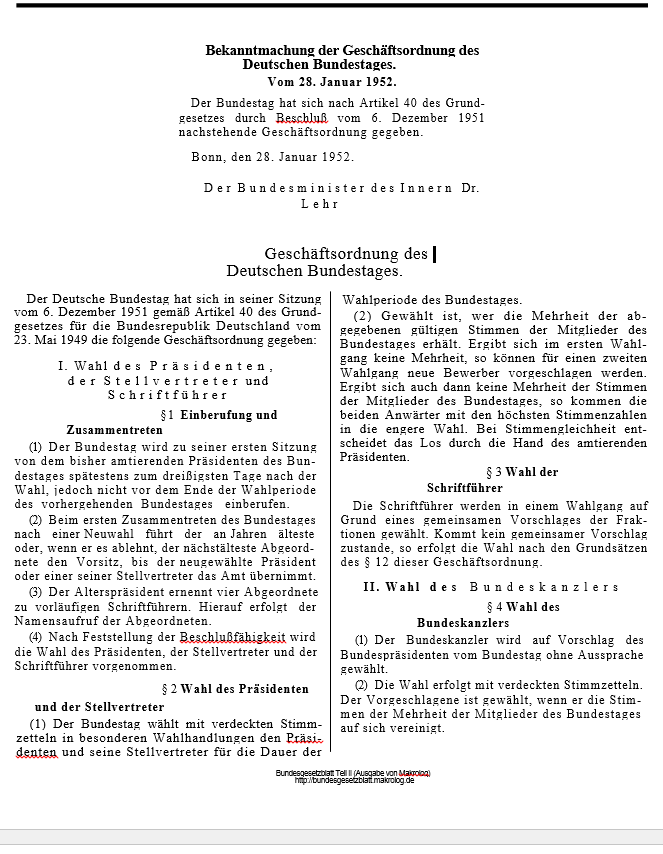
\includegraphics[height=0.4\textheight]{fig/fig1.png}
\end{center}

\emph{Figure 1: 1952 German Bundestag Standing Orders word-document}

\section{Document Consolidation}\label{document-consolidation}

In order to construct a data base consisting of all parliamentary
standing orders that were in force at a specific point in time
consolidated versions of the standing orders were needed. Consolidated
versions are complete versions with all changes that had occurred at a
specific date included in the body of the text.

However, there are often only few consolidated versions provided by
national parliaments. Changes to the standing orders are most of the
time published as amendments and only once in a while a full version of
the current text is issued. As a consequence, consolidated versions of
the standing orders for every date of change had to be constructed by
inserting manually the changes into the previous complete version.

\begin{center}
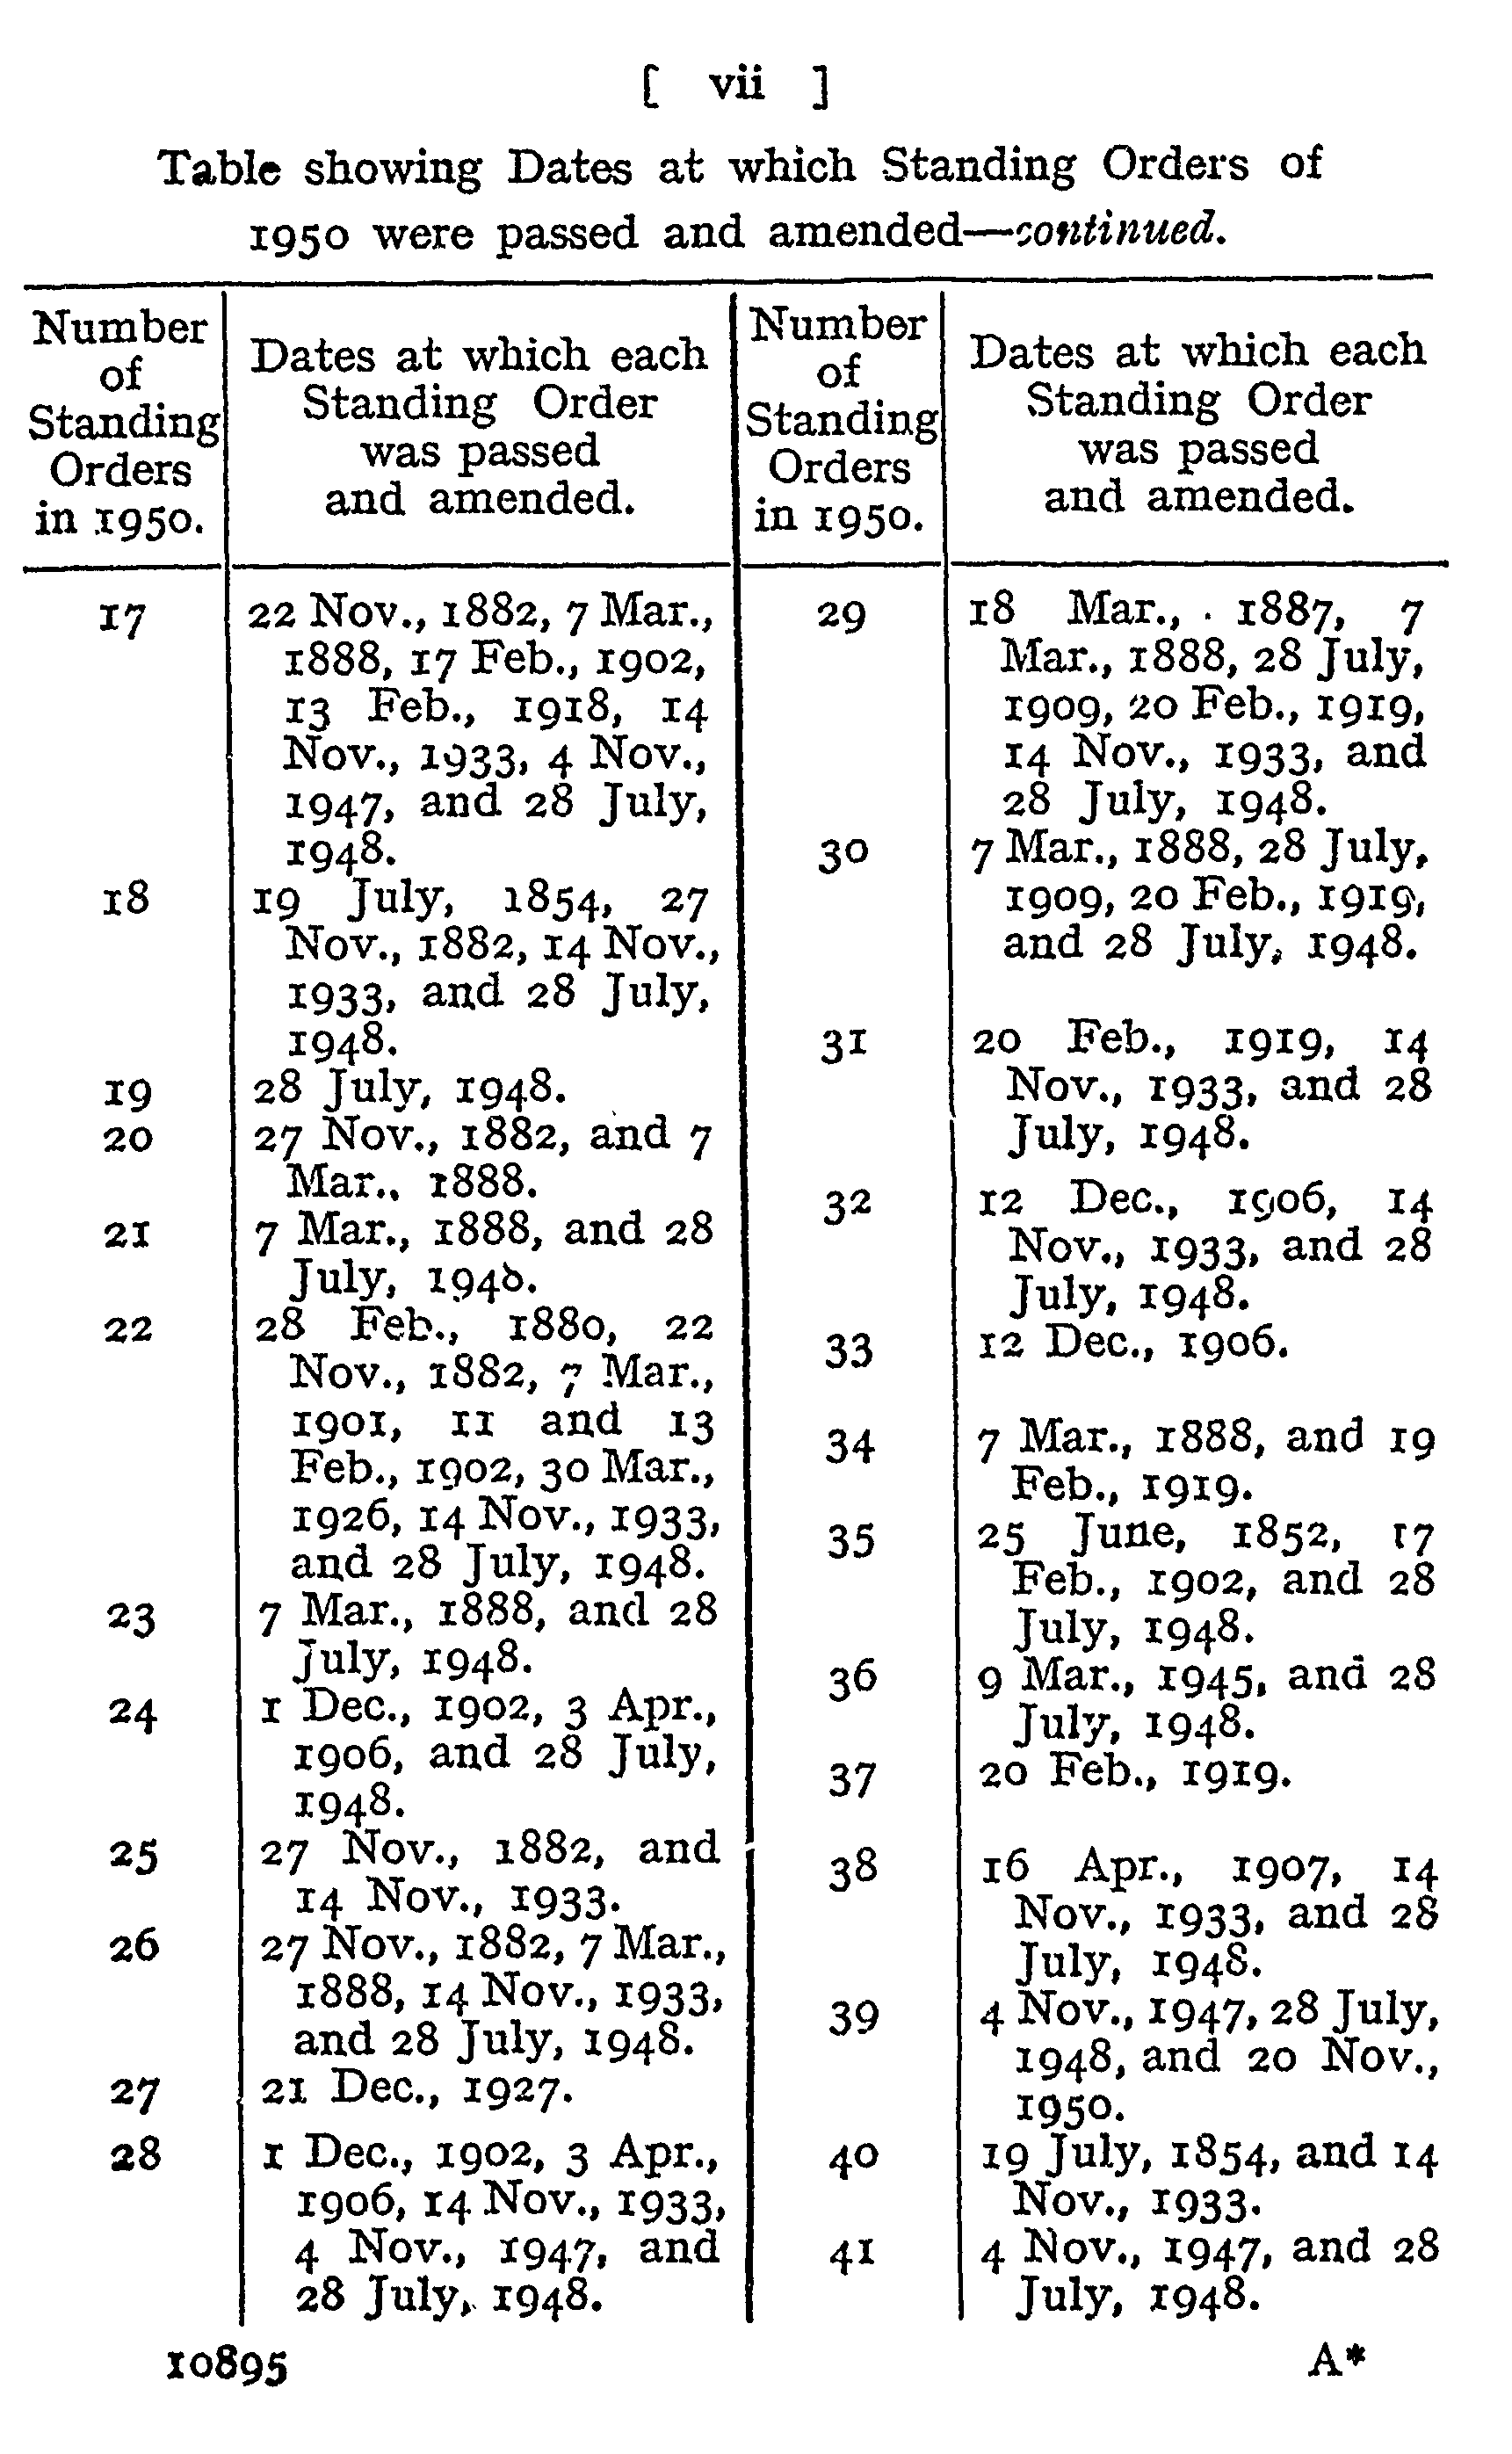
\includegraphics[height=0.4\textheight]{fig/fig1a.png}
\end{center}

\emph{Figure 2: List of ammendments to the 1950 SO UK, page 497}

\section{Document Cleaning}\label{document-cleaning}

The aim of this procedure was to identify and correct errors that had
occurred through the process of converting PDF-documents into
Word-documents. Another purpose was to put the cleaned versions of the
parliamentary standing orders in a standardized format while maintaining
the original structure of paragraphs. First of all, the oldest
consolidated version of Standing Orders was completely read through and
corrected manually. Typos, unnecessary line breaks, signs not belonging
to the text and everything going beyond the actual text of the standing
orders was deleted.

Next, a header containing information about the version such as the
dates of acceptance, promulgation and enactment of the version of the
standing orders was inserted. The version cleaned in this manner served
as reference version. In the following step the subsequent consolidated
version was compared to the reference version using the software DiffDoc
(in a later state of the cleaning process the software UltraCompare was
used instead). The software made it possible to easily identify
identical parts of the two versions that only contained few mistakes to
be corrected as well as parts that had been changed. The latter were
read completely and handled like the first version. After the cleaning
of the second version it served as new reference version for the
subsequent consolidated version of the standing orders. Alongside
cleaning the text, it was made sure that each sub-paragraph, headline or
other structuring element of the standing orders was given a single
line. Each element was separated by a line break; no element was allowed
to spread more than one line. The steps were repeated for all
consolidated versions. Throughout the procedure the PDF-versions of the
standing orders were considered in case of uncertainty regarding
cleaning decisions. In a last step the lines (representing text
elements) that were of non-relevant content (e.g.~headlines) were marked
by adding a special string at the start of the line (`\#§\#') to allow
the computer to automatically dismiss these lines later on.

\begin{center}
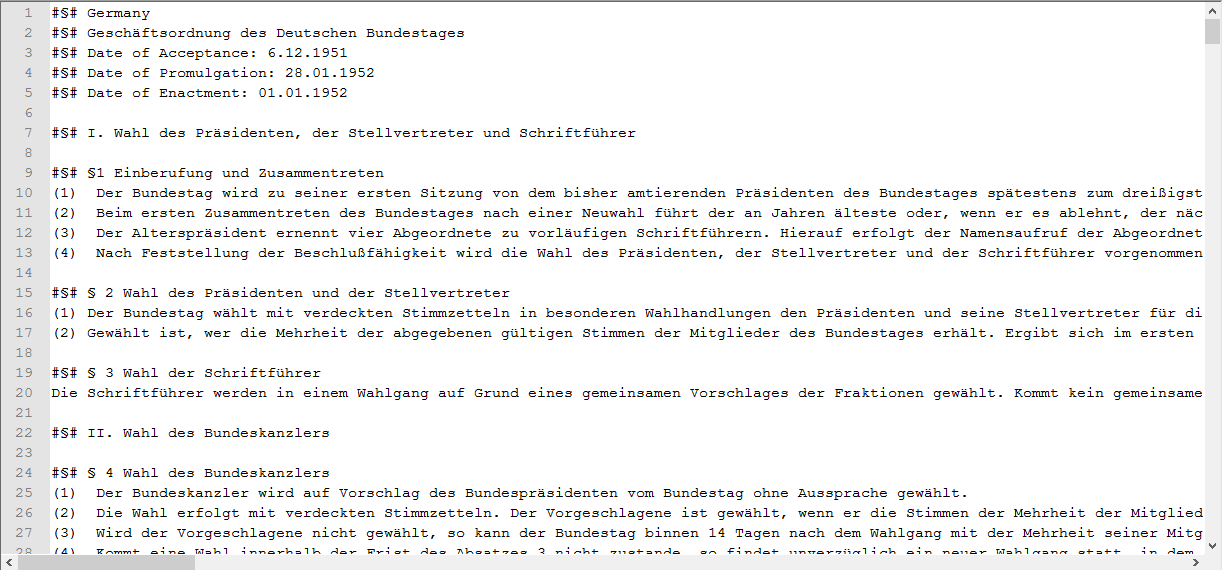
\includegraphics[width=\textwidth]{fig/fig2.png}
\end{center}

\emph{Figure 3: 1952 SO Germany plain-text version}

\begin{center}
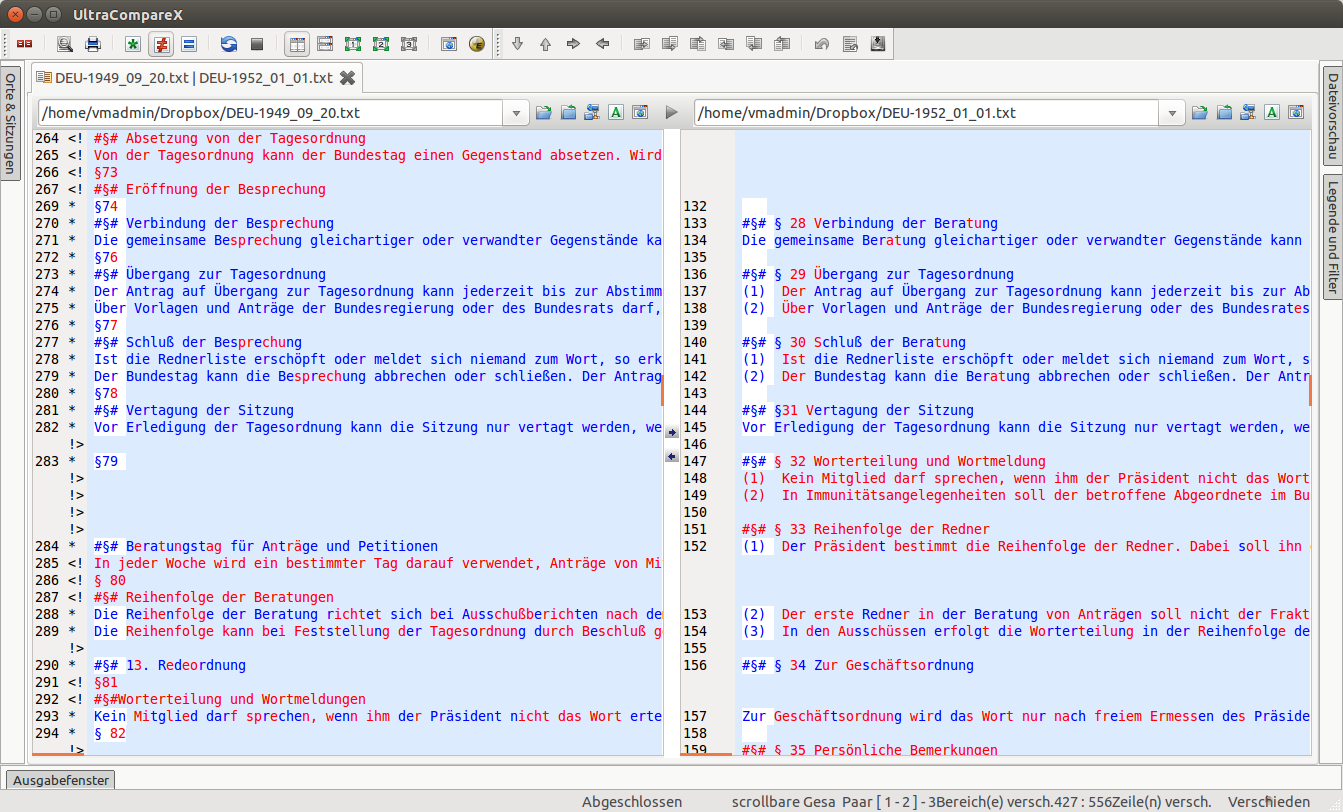
\includegraphics[height=0.4\textheight]{fig/fig3a.png}
\end{center}

\emph{Figure 4: Comparing Standing Orders versions with Ultra Compare}

\section{Linkage}\label{linkage}

Having generated complete, cleaned versions of the standing orders, the
next step was to further prepare the data so that the content of the
standing orders could be coded in an efficient manner and to get
information about what had or had not changed from one version to the
next. For this purpose changes in the standing orders between versions
were linked. This means that for each line of text (each relevant
sub-paragraph) it was recorded whether or not the line was deleted in
the version to come, got inserted in the current version, got changed or
simply stayed the same. The coding was done semi-automatically by first
letting an algorithm developed by the project and implemented in R
handle all non-relevant lines as well as those that were not changed.
Thereafter human coders went through all remaining text lines of two
subsequent versions to add there linkage information to the data-set.
For this another program implemented in R helped the coders by making
sure that: all lines were coded; the information was recorded correct
and alongside the text that was linked, coders were given suggestions
for possible matching lines similar to that under consideration. As the
linked files depicted the basis for later analyzes and coding, it was
crucial to differentiate between minor reformulations of paragraphs
(e.g.~mere orthographic reforms) and actual changes. In case of doubt
the supervisors were consulted.

The process of gathering link information between sub-paragraphs of
subsequent standing orders versions allows for distinguishing between
types of change (deletion, insertion, modification and no-change),
measuring its extent more precisely and to later transfer line codes
from one version of the standing orders to another so that all
sub-paragraphs (the selected coding entity) that were identical in two
versions got automatically the same code.

Furthermore, the use of an semi-automatic approach allows to use the
strengths of both computers and humans: computers are good at doing the
same stuff over and over again in the same and predictable way -
e.g.~finding identical lines, computing measures of similarity, saving
data always in the very same format -- while humans on the other hand
have a much better understanding of the content of text, might
understand intentions of the text authors and are more creative and
flexible -- e.g.~finding line pairs that might be not very similar based
on the sequence of characters or the distribution of words but in regard
to the things that are regulated within.

\begin{Shaded}
\begin{Highlighting}[]
\KeywordTok{library}\NormalTok{(stringr)}
\KeywordTok{library}\NormalTok{(diffr)}

\CommentTok{# defining text}
\NormalTok{old <-}\StringTok{ }\KeywordTok{str_split}\NormalTok{(}\StringTok{"Three kind mice, see how they run!}\CharTok{\textbackslash{}n}\StringTok{They all ran after the farmer's wife,}\CharTok{\textbackslash{}n}\StringTok{Who cut off their tails with the carving knife,}\CharTok{\textbackslash{}n}\StringTok{Did you ever see such a thing in your life?}\CharTok{\textbackslash{}n}\StringTok{As three blind mice.}\CharTok{\textbackslash{}n}\StringTok{End"}\NormalTok{, }\StringTok{"}\CharTok{\textbackslash{}n}\StringTok{"}\NormalTok{)}
\NormalTok{new <-}\StringTok{ }\KeywordTok{str_split}\NormalTok{(}\StringTok{"Three blind mice, see how they run!}\CharTok{\textbackslash{}n}\StringTok{They all ran after the farmer's wife,}\CharTok{\textbackslash{}n}\StringTok{they took out some cheese,}\CharTok{\textbackslash{}n}\StringTok{and they cut her a slice,}\CharTok{\textbackslash{}n}\StringTok{Did you ever see such a sight in your life}\CharTok{\textbackslash{}n}\StringTok{as three kind mice?"}\NormalTok{, }\StringTok{"}\CharTok{\textbackslash{}n}\StringTok{"}\NormalTok{)}

\CommentTok{# calculating distances, aligning text, determining change types}
\NormalTok{res <-}\StringTok{ }\KeywordTok{diffr}\NormalTok{(old, new, }\DataTypeTok{dist=}\StringTok{"bow"}\NormalTok{)}

\CommentTok{# distance matrix}
\NormalTok{res$distance_matrix}
\end{Highlighting}
\end{Shaded}

\begin{verbatim}
##      [,1] [,2] [,3] [,4] [,5] [,6]
## [1,]    2   15   10   11   15    7
## [2,]   15    0   13   14   18   12
## [3,]   16   15   14   13   19   13
## [4,]   15   18   15   14    2   14
## [5,]    7   12    9   10   14    4
## [6,]    8    9    6    7   11    5
\end{verbatim}

\begin{Shaded}
\begin{Highlighting}[]
\CommentTok{# resulting alignment and change type}
\NormalTok{res$alignment_df}
\end{Highlighting}
\end{Shaded}

\begin{verbatim}
##   lnr1 lnr2 distance      type
## 1    1    1        2    change
## 2    2    2        0 no change
## 3    3    4       13    change
## 7   NA    3        5 insertion
## 4    4    5        2    change
## 5    5    6        4    change
## 6    6   NA        1  deletion
\end{verbatim}

\emph{Code Snippet 1: Text comparison with own software written in R}

\begin{center}
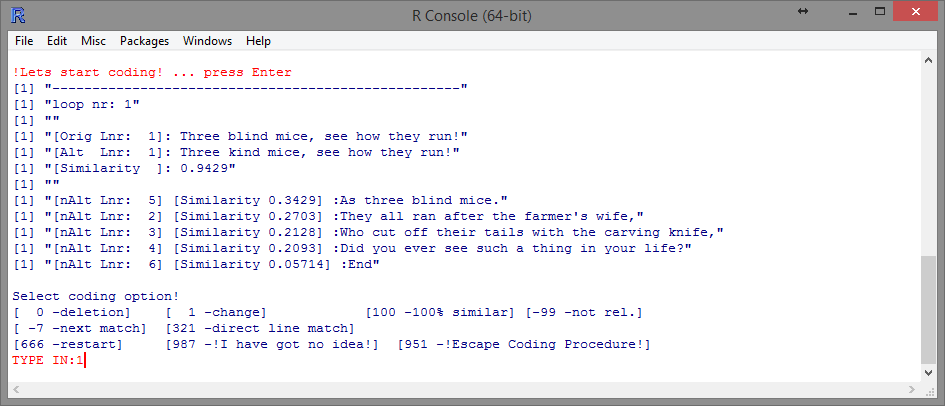
\includegraphics[height=0.4\textwidth]{fig/linkage.png}
\end{center}

\emph{Figure 5: R Software with commandline interface for linking parts
of two version of Standing Orders}

\section{Minority-Majority-Change
Coding}\label{minority-majority-change-coding}

\section{Corpus Coding}\label{corpus-coding}

Based on the linked versions of the standing orders the content could be
coded. The intention of the so called corpus coding process was to
assign a single code expressing the content to every legal sub-paragraph
of every version of the standing orders.

The coding scheme comprises 80 different single codes belonging to ten
different categories (law-making, special decision procedures other than
regular law-making, relationship to government, relationship to external
offices/institutions apart from the government, generating publicity,
internal organization of parliament, change and interpretation of the
standing orders, general rules regarding formation and legislative
session/discontinuity, final provisions, miscellaneous (cannot be coded
otherwise)).

Apart from the codes the coding manual encompasses general rules for
coding. As every sub-paragraph got only one code the coders had to
decide which code suites best even if several different codes could be
assigned to a sub-paragraph. These decisions were based on a specific
hierarchy of codes. Rules which concern the interaction of two actors
were attributed to the actor which takes the active part if he has
discretion regarding this action. Regular law-making was considered more
important than other decision procedures if they were treated together
in one sub-paragraph. A further general coding rule was to take the
overall context into account instead of just looking at a specific
regulation.

Like the other coding processes corpus coding was done
semi-automatically with a self-written program implemented in R. Human
coders went through the oldest version of the standing orders and
assigned the appropriate codes from the coding scheme to every text line
to create one fully coded version. The next step was to transfer these
codes to the other versions. As in the linking procedure text lines that
have stayed exactly the same from one version to the following had been
identified and linked, the R program automatically assigned the same
codes to them. So the coders only had to go through the not coded text
lines of the subsequent version of the standing orders (that is the
passages that had been changed between two versions) and code them
manually. Then, the new codes were transferred. The coders proceeded in
this way until all versions of the standing orders were completely coded
with regard to their content.

The original standing orders of national parliaments are usually only
published in the language of the country. Thus, coders were recruited
who were either native speakers or non-native speakers with very high
language proficiency. Good knowledge about the government system of the
countries was a further requirement. As corpus coding was a very
demanding task, all coders got intensive training. First, the coders
familiarized themselves with the coding manual, the different categories
and coding rules. Next, the new coders practiced through joint coding
with experienced coders. After this, the coders coded the most recent
version of the standing orders and compared their results to a master
version. Usually the most recent versions of the standing orders are
also issued in English. These versions had been coded by those
responsible for the project and served as master versions. On condition
that coders mastered this task they could start coding on their own.
Throughout the coding process ambiguities and problems were solved in
joint discussion with the project coordinators. If it was necessary,
supplementary documents such as constitutions and information from the
webpages of the national parliaments were considered to check coding
decisions.

\section{Appendix}\label{appendix}

\subsection{Manual for Text Cleansing}\label{manual-for-text-cleansing}

\subsection{Manual for Text
Cosolidation}\label{manual-for-text-cosolidation}

\subsection{Coding Scheme for Corpus
Coding}\label{coding-scheme-for-corpus-coding}

\subsubsection{Basic Intuition:}\label{basic-intuition}

Each and every code is exclusive, meaning that one sub-paragraph needs
to have one code but one code only. For some codes there are notes on
how to decide between multiple codes which may seem appropriate.
Sometimes even the coding rules and additional notes will not help to
decide between codes. In this case please let us know. Every decision
accompanied by doubt should be documented.

\subsubsection{Further rules of the
game:}\label{further-rules-of-the-game}

\begin{itemize}
\item
  Often sub-paragraphs can be coded differently, depending on whether or
  not one takes into consideration the overall context of the rule or
  the more specific regulation. If in doubt, code based on the overall
  context. Example: §14 GOBT: president grants vacation time → coded as
  rights and obligations of individual members of parliament if one
  takes into account the general context (652) and not as responsibility
  of the president (6212).
\item
  Rules which concern the interaction of two actors are attributed to
  the actor which takes the active part if he has discretion regarding
  this action. Example: §62 (2) GOBT: The plenary can request report of
  committee → coded as recall through the plenary (124) and not as
  report of committee to the plenary (134).
\item
  The right of those initiating a bill or law to be present at the
  committee meetings is coded as general right of individual members of
  parliament (652).
\end{itemize}

\subsubsection{Scheme}\label{scheme}

\textbf{(1) Law Making}

~

\emph{Note: SPs that refer to both the plenary sessions and committees
are coded as 12x; SPs dealing with both law-making and special decision
procedures are coded as 1xx.}

\begin{itemize}
\tightlist
\item
  \textbf{11 Bills and Motions}

  \begin{itemize}
  \tightlist
  \item
    111 types of bills and motions; printing and distribution of bills
    and motions to MPs
  \item
    112 right to initiate bills and motions
  \item
    113 restrictions and deadlines (if not assignable to more specific
    category, e.g.~code 121; 32; 134)
  \item
    114 legislative planning (concerns the whole term- general schedule)
  \end{itemize}
\item
  \textbf{12 Treatment of bills and motions in the plenary} \emph{(Note:
  SPs including all stages of the treatment of bills and motions are
  coded as votes in the plenary (123); SPs which determine the subject
  of debate and vote are coded as subject of vote (123).)}

  \begin{itemize}
  \tightlist
  \item
    121 debate in the plenary
  \item
    122 right of amendment in the plenary
  \item
    123 subject of vote, rules of vote (including quorum), voting
    technology in the plenary
  \item
    124 the plenary as Committee of the Whole House \emph{(Note: SPs
    referring to both committees and Committee of the Whole House are
    coded as committees (not 124 but 13x).)}
  \item
    125 referral to committee, withdrawal from committee
  \end{itemize}
\item
  \textbf{13 Treatment of bills and motions in committee} \emph{(Note:
  SPs including all stages of the treatment of bills and motions in
  committee are coded as votes in committee (133); SPs which determine
  both the subject of debate and the subject of vote are coded as
  subject of vote in committee (133).)}

  \begin{itemize}
  \tightlist
  \item
    131 debate in committee (including hearing)
  \item
    132 amendment rights in committee
  \item
    133 subject of vote, rules of vote (including quorum), voting
    technology in committee
  \item
    134 report to the plenary
  \end{itemize}
\end{itemize}

\textbf{(2) Special Decision Procedures other than Regular Law-Making}

~

\emph{Note: SPs which concern multiple special decision procedures apart
from regular law-making are coded as follows: highest priority is given
to constitutional matters, second highest priority is given to financial
laws and budgeting, third highest priority is given to EU policy and
fourth highest priority is given toforeign policy.}

\begin{itemize}
\tightlist
\item
  \textbf{21 constitutional change and amendment}
\item
  \textbf{22 financial laws} (money bills) and budgeting
\item
  \textbf{23 foreign policy} (e.g.~approval of law of nations,
  declaration of war \emph{Note: If foreign policy and EU is treated
  together, the SP is coded as EU (241, 242, 243 or 244).})
\item
  \textbf{24 EU} \emph{(Note: If foreign policy and EU is treated
  together, the SP is coded as EU (241, 242, 243 or 244))}

  \begin{itemize}
  \tightlist
  \item
    241 treatment of EU-bills and motions
  \item
    242 EU-committee: election and resignation
  \item
    243 instructions to the government concerning EU decisions
  \item
    244 further rights of participation in EU matters (e.g.~debates
    about EU topics not based on EU bills and motions, reaction to
    violations of subsidiary principle)
  \end{itemize}
\item
  \textbf{25 general rules on elections in parliament} (if not coded as
  election of government (31), or election of specific officials (411;
  421; 441; 6211; 6221; 632))
\item
  \textbf{26 further special decision procedures} leading to a decision,
  e.g.~resolution, or leading to a decree/act/bylaw (not mere debate or
  question time) but cannot be coded as regular law-making nor special
  decision procedures (21-24)
\item
  \textbf{27 procedures concerning laws that are hierarchically situated
  between regular laws and constitutional laws} (above regular laws;
  e.g.~organic laws in Spain)
\item
  \textbf{28 emergency legislation}
\item
  \textbf{29 relationship to sub-national level} (law-making, rights of
  participation of sub-national level)
\end{itemize}

\textbf{(3) Relationship to Government}

~

\emph{Note: If vote of no confidence and vote of confidence is treated
together, the SP is coded as vote of no confidence (32).}

\begin{itemize}
\tightlist
\item
  \textbf{31 election of government / mandatory investiture vote; entry
  into office}
\item
  \textbf{32 vote of no confidence / government resignation}
\item
  \textbf{33 vote of confidence}
\item
  \textbf{34 instructions to government, involvement of members of
  government in parliamentary activities} (rights to compel witnesses
  {[}usually right of parliament against members of government{]}, right
  to speak {[}usually members of government's right{]}, request of
  information about state of execution of decisions of parliament)
\end{itemize}

\textbf{(4) Relationship to External Offices/Institutions apart from the
Government}

\begin{itemize}
\tightlist
\item
  \textbf{41 parliamentary support bodies (e.g.~general accounting
  office, ombudsman,\ldots{})}

  \begin{itemize}
  \tightlist
  \item
    411 election and resignation
  \item
    412 competences and resources of external offices/institutions;
    relations to parliament (e.g.~reports, questions, \ldots{})
  \end{itemize}
\item
  \textbf{42 head of state}

  \begin{itemize}
  \tightlist
  \item
    421 election and resignation
  \item
    422 relation to parliament (if not coded as law-making (141, 144))
  \end{itemize}
\item
  \textbf{43 second chamber (if not coded as law-making (142))}
\item
  \textbf{44 constitutional courts}

  \begin{itemize}
  \tightlist
  \item
    441 election and resignation
  \item
    442 relation to parliament (if not coded as law-making (145))
  \end{itemize}
\item
  \textbf{45 other external offices}
\end{itemize}

\textbf{(5) Generating Publicity}

\begin{itemize}
\tightlist
\item
  \textbf{51 general rules regarding debate} (e.g.~time allotted for
  speaking, proportional representation of parties during debate,
  closure of debate)
\item
  \textbf{52 debates outside of law-making} (e.g.~topical hours
  \ldots{})
\item
  \textbf{53 question rights}
\item
  \textbf{54 petitions and petition committee}
\item
  \textbf{55 relationship to media and citizens} (e.g.~parliamentary TV,
  accreditation of journalists, publicity of meetings, admissibility of
  visitors); regulation of matters of confidentiality
\item
  \textbf{56 protocols and parliamentary documents; forwarding of
  documents and decisions to other bodies}
\end{itemize}

\textbf{6 Internal Organization of Parliament}

\begin{itemize}
\tightlist
\item
  \textbf{61 plenary}

  \begin{itemize}
  \tightlist
  \item
    611 agenda setting and removal of items from the agenda (general
    rules which are not specifically regulated under 114)
  \item
    612 chairing of meetings and measures to uphold order
  \item
    613 sitting times \emph{(Note: When members are to be present inside
    the parliament)}
  \end{itemize}
\item
  \textbf{62 parliamentary presiding bodies}

  \begin{itemize}
  \tightlist
  \item
    621 president of parliament, vice presidents, secretaries and clerks

    \begin{itemize}
    \tightlist
    \item
      6211 election, resignation and internal decision rules
    \item
      6212 responsibilities \emph{(Note: if not coded as more specific
      category (e.g.~612), Try to code in regard to the topic at first -
      6212 only when no code corresponds)}
    \end{itemize}
  \item
    622 council of elders or similar coordination body \emph{(Note: The
    council of elders can be distinguished from the Presidency of
    Parliament (621) insofar as representatives of the parliamentary
    party groups are explicitly included.)}

    \begin{itemize}
    \tightlist
    \item
      6221 composition, election, resignation, internal decision rules
    \item
      6222 responsibilities (if not coded as more specific category
      (e.g.~612))
    \end{itemize}
  \end{itemize}
\item
  \textbf{63 committees} (if not coded as more specific category
  (e.g.~13; 24; 54; 55; 72))

  \begin{itemize}
  \tightlist
  \item
    631 general regulations regarding types of committees
  \item
    632 membership and committee jurisdiction (area of influence-control
    .g. finance, economy, agriculture\ldots{})
  \item
    633 formal organizational units of committee \emph{(Note: e.g.~chair
    of committee, sub-committees, staff; This is about the appointment
    and election of the organizational units within committees and NOT
    about their responsibilities.)}
  \item
    634 agenda and procedures (details on how decisions are taken)
    within committees (if not coded as law-making (13))
  \item
    635 relations to other bodies

    \begin{itemize}
    \tightlist
    \item
      6351 relation to plenary (if not coded as 124; 134; 34)
    \item
      6352 relation to other committees
    \end{itemize}
  \item
    636 investigative competencies of regular committees (NOT committees
    of inquiry (637))

    \begin{itemize}
    \tightlist
    \item
      637 committee of inquiry
    \item
      638 enquête commission
    \end{itemize}
  \item
    639 other special committees which are not explicitly referenced in
    this coding manual \emph{(Note: e.g.~oversight committees in
    Switzerland; Otherwise referenced are: EU-committee (242); committee
    of inquiry (637); petition committee (54); standing order committee
    (usually 72); council of elders or similar coordination body (622).
    Exception: committees which deal exclusively with the confirmation
    of the elections of members of parliament are coded as 651.)}
  \end{itemize}
\item
  \textbf{64 parliamentary party groups}

  \begin{itemize}
  \tightlist
  \item
    641 formation of parliamentary party groups
  \item
    642 rights and obligations of parliamentary party groups (if not
    coded more specifically as e.g.~112; 51; 52; 53)
  \item
    643 financial and staff resources
  \end{itemize}
\item
  \textbf{65 individual members of parliament}

  \begin{itemize}
  \tightlist
  \item
    651 election, entry into office, resignation, incompatibilities,
    legal status, immunity, indemnity
  \item
    652 rights and obligations of individual members of parliament (if
    not coded more specifically as e.g.~112; 51; 52; 53)
  \item
    653 salary, financial and staff resources
  \end{itemize}
\item
  \textbf{66 opposition}
\item
  \textbf{67 special bodies for emergency situations}
\item
  \textbf{68 parliamentary administration}
\end{itemize}

\textbf{7 Change and Interpretation of the Standing Orders}

\begin{itemize}
\tightlist
\item
  \textbf{71 rules regarding changing the standing orders}
\item
  \textbf{72 rules regarding interpretation of and deviation from
  standing orders}
\item
  \textbf{73 debate about standing orders and motions regarding the
  standing orders}
\end{itemize}

\textbf{8 General Rules Regarding Formation and Legislative Session;
Discontinuity}

\textbf{9 Final Provisions}

\textbf{10 Miscellaneous} (cannot be coded otherwise)

\textbf{999 Footnotes and Titles Without Relevant Content}

\end{document}
